% Apêndice
\apendice
\chapter{Primeiro apêndice}

\begin{figure}
  \centering
    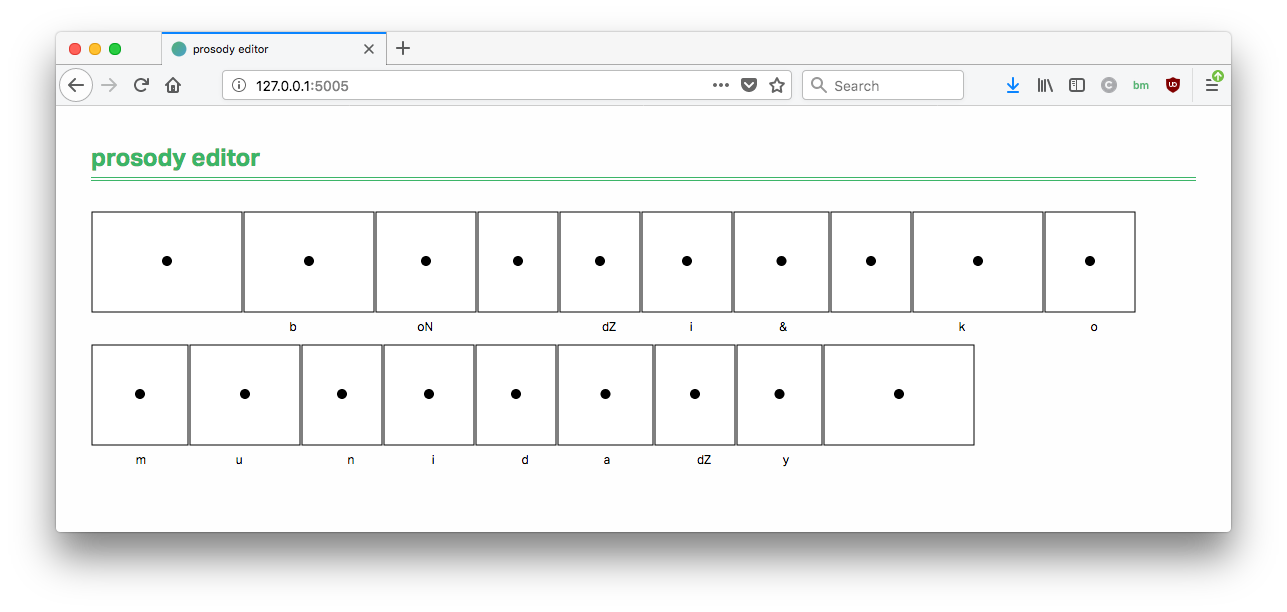
\includegraphics[width=1\textwidth]{Imagens/editor.png}
  \caption{Editor gráfico}
\end{figure}

\begin{lstlisting}[caption=Servidor, label=servidor, language=Python]
import sqlite3
import sampa_mbrola
from flask import Flask, g, jsonify, render_template, abort, request
from flask_cors import CORS

app = Flask(__name__)
CORS(app)

@app.route('/api/espeak', methods=['POST'])
def frontend():
    text = request.form['text']
    converter = sampa_mbrola.Converter()
    sentence = converter.convert_sentence(text)
    return jsonify(sentence.dictify())

@app.route('/api/mbrola', methods=['GET'])
def mbrola(page):
    pass

if __name__ == '__main__':
    app.run(debug=True)
\end{lstlisting}

\begin{lstlisting}[caption=Conversor eSpeakNG-MBROLA, label=conversao, language=Python]
import sys
import re
import subprocess
import random
import json
from collections import OrderedDict
from typing import List

def flatten(lst: list):
    return [item for sublist in lst for item in sublist]

class Phone():
    def __init__(
            self,
            phone_sampa: str,
            phone_mbrola: str,
            duration: int,
            pitch_changes: list
    ):
        self.phone_sampa = phone_sampa
        self.phone_mbrola = phone_mbrola
        self.duration = duration
        self.pitch_changes = pitch_changes

    def as_line(self):
        return "{} {} {}".format(
            self.phone_mbrola,
            self.duration,
            " ".join([str(item) for item in flatten(self.pitch_changes)])
        )

class Sentence():
    def __init__(self, phones: List[Phone]=None):
        if phones is None:
            self.phones = []
        else:
            self.phones = phones

    def mbrola_phones(self):
        return [phone.phone_mbrola for phone in self.phones]

    def dictify(self):
        return [vars(phone) for phone in self.phones]

    def __repr__(self):
        return "\n".join([phone.as_line() for phone in self.phones])


class Converter():
    def __init__(self):
        self.load_sampa_mbrola()
        self.load_durations()

    def load_sampa_mbrola(self):
        equivs = {}
        with open("sampa_mbrola.tbl") as f:
            for line in f:
                k, v, _ = line.split()
                equivs[k] = v

        self.equivs = OrderedDict(
            sorted(equivs.items(), key=lambda t: -len(t[0])))

    def load_durations(self):
        durations = {}
        with open("durations.tbl") as f:
            for line in f:
                k, v = line.split()
                durations[k] = v

        self.durations = durations

    def convert_phoneme(self, sentence: str) -> tuple:
        """Returns first phone from the sentence"""

        if sentence[0] == " ":
            return ("_", 1)
        elif self.equivs:
            # s is a special case, needs to peek next
            if sentence[0] == "s":
                if sentence[1] in "aeiou&":
                    return ("s", 1)

            for equiv in self.equivs.items():

                if re.match(re.escape(equiv[0]), sentence):
                    # print("match:", equiv[0], phoneme, "=", equiv[1])
                    return (equiv[1], len(equiv[0]))

        # print("didn't match", phoneme)
        return (phoneme[0], 1)

    def get_duration(self, phoneme: str) -> int:
        if self.durations and phoneme in self.durations:
            return self.durations[phoneme]
        else:
            return 100

    def convert_sentence(self, input_str: str) -> Sentence:
        sentence = Sentence()
        sentence.phones.append(Phone(" ", "_", 150, [[50, 150]]))

        ignored = ["@", "\n", ",", "'", "^", ";"]

        sampa = self.text_to_sampa(input_str)
        sampa = sampa.replace("'", "")
        print(";; ", sampa)

        while sampa:
            if sampa[0] not in ignored:
                converted = self.convert_phoneme(sampa)
                phone_sampa = sampa[:converted[1]]
                sampa = sampa[converted[1]:]

                duration = self.get_duration(converted[0])
                phone = Phone(
                    phone_sampa = phone_sampa,
                    phone_mbrola = converted[0],
                    duration = int(duration),
                    pitch_changes = [[50, 150]] # percentage, Hz
                )

                sentence.phones.append(phone)
            else:
                sampa = sampa[1:]

        sentence.phones.append(Phone(" ", "_", 150, [[50, 150]]))
        return sentence

    def text_to_sampa(self, sentence: str) -> str:
        espeak_str = "espeak-ng -v pt-br '{}' -x -q".format(sentence)

        p = subprocess.Popen(espeak_str, stdout=subprocess.PIPE, shell=True)
        (output, err) = p.communicate()
        p_status = p.wait()
        output = output.decode("utf-8")
        output = output.replace("\n", "").strip()
        return output


if __name__ == "__main__":
    converter = Converter()

    for line in sys.stdin:
        print(";;", line)
        print(converter.convert_sentence(line))
\end{lstlisting}

\begin{lstlisting}[caption=Editor gráfico, label=editorjs, language=Python]
var app = new Vue({
  el: '#app',
  data: {
    phones: [],
    height: 300
  },
  mounted: function() {
    var self = this;
    const requestURL = "http://127.0.0.1:5000/api/espeak";
    let XHR = new XMLHttpRequest();
    let FD  = new FormData();

    FD.append("text", "Bom dia, comunidade");

    XHR.open("POST", requestURL);
    XHR.send(FD);

    XHR.onreadystatechange = function() {
      if (XHR.readyState === XMLHttpRequest.DONE) {
        if (XHR.status === 200) {
          const results = JSON.parse(XHR.responseText);
          self.phones = results;
        }
      }
    };
  },
  computed: {
    totalDuration: function() {
      let durations = this.phones.map((phone) => phone.duration);
      console.log(durations.reduce((acc, val) => acc + val, 0));
      return durations.reduce((acc, val) => acc + val, 0);
    }
  }
});
\end{lstlisting}

\begin{lstlisting}[caption=Exemplo de resposta para \emph{endpoint} do eSpeakNG, label=espeakpost, language=Python]
[
  {
    "duration": 150,
    "phone_mbrola": "_",
    "phone_sampa": " ",
    "pitch_changes": [[50, 150]
    ]
  },
  {
    "duration": 80,
    "phone_mbrola": "n",
    "phone_sampa": "n",
    "pitch_changes": [[50, 150]]
  },
  {
    "duration": 110,
    "phone_mbrola": "u",
    "phone_sampa": "U",
    "pitch_changes": [[50, 150]]
  },
  ...
  {
    "duration": 150,
    "phone_mbrola": "_",
    "phone_sampa": " ",
    "pitch_changes": [[50, 150]]
  }
]
\end{lstlisting}

\begin{lstlisting}[caption=Exemplo de resposta para \emph{endpoint} do MBROLA, label=mbrolaget, language=Python]
{
  "mp3_file": "07acc5c4ba924294.mp3"
}
\end{lstlisting}

\begin{lstlisting}[caption=Gerador de f0 a partir do modelo INTSINT, label=intsintpy, language=Python]
from math import sqrt

def intsint(labels: list, key: float = 220.0, range: float = 1.0):
    if labels[0] not in ["T", "M", "B"]:
        raise ValueError("First item in list can't be relative")

    freq_t = key * sqrt(2 ** range)
    freq_m = key
    freq_b = key / sqrt(2 ** range)

    freqs = []

    for idx, l in enumerate(labels):
        if l == "T":
            freqs.append(freq_t)
        elif l == "M":
            freqs.append(freq_m)
        elif l == "B":
            freqs.append(freq_b)
        elif l == "H":
            freqs.append(sqrt(labels[idx - 1]) * freq_t)
        elif l == "S":
            freqs.append(labels[idx - 1])
        elif l == "L":
            freqs.append(sqrt(labels[idx - 1]) * freq_b)
        elif l == "U":
            freqs.append(sqrt(labels[idx - 1]) * sqrt(labels[idx - 1] * freq_t))
        elif l == "D":
            freqs.append(sqrt(labels[idx - 1]) * sqrt(labels[idx - 1] * freq_b))
\end{lstlisting}
